% ============================================================
% BEAMER PRESENTATION: Time-Varying Exposure and Systemic Risk
% ============================================================
\documentclass[10pt,aspectratio=169]{beamer}

% Theme and color setup
\usetheme{Madrid}
\usecolortheme{default}
\setbeamertemplate{navigation symbols}{}
\setbeamertemplate{footline}[frame number]

% Packages
\usepackage{amsmath,amssymb}
\usepackage{booktabs}
\usepackage{graphicx}
\usepackage{tikz}
\usetikzlibrary{arrows,shapes,positioning,calc}
\usepackage{multirow}

% Custom colors
\definecolor{darkblue}{RGB}{0,51,102}
\definecolor{lightblue}{RGB}{51,102,153}
\definecolor{orange}{RGB}{255,102,0}
\definecolor{gray}{RGB}{128,128,128}

\setbeamercolor{structure}{fg=darkblue}
\setbeamercolor{frametitle}{bg=darkblue,fg=white}
\setbeamercolor{title}{bg=darkblue,fg=white}

% Title information
\title[Time-Varying Exposure \& Systemic Risk]{Time-Varying Exposure and Systemic Risk:\\Amortisation Schedules in Sector-Apportioned Intensity Models}
\author{ Devang Sinha \and Siddharth Kamlesh Sharma \and Shashi Jain \and Srikanth K. Iyer}
\institute{}
\date{}

\begin{document}

% ============================================================
% TITLE SLIDE
% ============================================================
\begin{frame}
\titlepage
\end{frame}

% ============================================================
% OUTLINE
% ============================================================
\begin{frame}{Outline}
\tableofcontents
\end{frame}

% ============================================================
% SECTION 1: MOTIVATION
% ============================================================
\section{Motivation}

\begin{frame}{The Problem: Static Exposure Assumptions}

\begin{columns}[T]
\begin{column}{0.48\textwidth}
\textbf{Standard Credit Risk Models}
\begin{itemize}
\item Treat loss at default as uniform draw
\item Assume constant exposure (EAD)
\item Implicitly: full loss given default
\end{itemize}

\vspace{1em}
\textbf{Reality}
\begin{itemize}
\item Outstanding principal \emph{evolves}
\item Repayment schedules differ
\item Timing matters
\end{itemize}
\end{column}

\begin{column}{0.48\textwidth}
\begin{center}
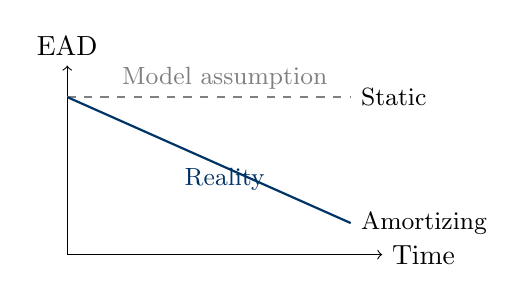
\begin{tikzpicture}[scale=0.8]
% Axes
\draw[->] (0,0) -- (5,0) node[right] {Time};
\draw[->] (0,0) -- (0,3) node[above] {EAD};

% Static exposure (dashed)
\draw[dashed, thick, gray] (0,2.5) -- (4.5,2.5) node[right, black] {\small Static};

% Declining exposure
\draw[thick, darkblue] (0,2.5) -- (4.5,0.5) node[right, black] {\small Amortizing};

% Annotations
\node[gray] at (2.5,2.8) {\small Model assumption};
\node[darkblue] at (2.5,1.2) {\small Reality};
\end{tikzpicture}
\end{center}

\vspace{1em}
\alert{Gap:} How does repayment structure affect \emph{systemic risk}?
\end{column}
\end{columns}

\end{frame}

\begin{frame}{Sector-Apportioned Intensity Framework}

\textbf{Base Model} \cite{sinha2025}:
\vspace{-0.3em}
\begin{equation*}
\lambda^A_t = X^A + \sum_{j=1}^{J} w^{Aj}\,Y^j_t
\end{equation*}

\begin{itemize}
\item $X^A$: idiosyncratic intensity (constant)
\item $Y^j_t$: sector-$j$ intensity (CIR dynamics with loss feedback)
\item $w^{Aj}$: exposure weight to sector $j$
\end{itemize}

\vspace{1em}
\textbf{Contagion Mechanism:}
\begin{itemize}
\item Each default triggers jump: $\Delta Y^j = \delta^{Aj} \ell / P$
\item Loss-driven feedback $\rightarrow$ self-exciting defaults
\item Generates clustering characteristic of credit crises
\end{itemize}

\end{frame}

\begin{frame}{Our Contribution}

\textbf{We extend the model along two dimensions:}

\vspace{1em}
\begin{enumerate}
\item \textbf{Time-varying EAD:}
\begin{equation*}
\ell^A = \mathrm{LGD}^A \cdot \alert{E^A(\tau^A)}
\end{equation*}
where $E^A(t)$ follows contractual repayment schedule

\vspace{1em}
\item \textbf{Stochastic LGD:}
\begin{equation*}
\mathrm{LGD}^A \sim \mathrm{Beta}(4.5, 5.5) \quad \text{(mean 45\%, std 15\%)}
\end{equation*}
\end{enumerate}

\vspace{1em}
\textbf{Study four canonical amortisation structures:}
\begin{itemize}
\item Bullet, Linear (Italian), French, Negative Amortisation
\end{itemize}

\end{frame}

% ============================================================
% SECTION 2: AMORTISATION SCHEDULES
% ============================================================
\section{Amortisation Schedules}

\begin{frame}{Four Canonical Repayment Structures}

\begin{columns}[T]
\begin{column}{0.48\textwidth}
\textbf{1. Bullet}
\begin{itemize}
\item No principal repayment until maturity
\item $E_B(t) = P$ for all $t < T$
\item Maximum credit exposure
\end{itemize}

\vspace{0.5em}
\textbf{2. Linear (Italian)}
\begin{itemize}
\item Equal principal installments
\item $E_L(t) = P(1 - t/T)$
\item Uniform decline
\end{itemize}

\vspace{0.5em}
\textbf{3. French (Constant-Annuity)}
\begin{itemize}
\item Constant total payment
\item Early: mostly interest
\item Most residential mortgages
\end{itemize}

\vspace{0.5em}
\textbf{4. Negative Amortisation}
\begin{itemize}
\item Interest capitalizes
\item $E_N(t) = P(1+r)^t > P$
\item Growing exposure
\end{itemize}
\end{column}

\begin{column}{0.48\textwidth}
\includegraphics[width=\textwidth]{figures/ead_profiles.png}

\vspace{0.5em}
\small
\textbf{Parameters:} $P=10$, $T=5$ years, $r=12\%$, monthly payments
\end{column}
\end{columns}

\end{frame}

\begin{frame}{Cumulative Exposure Mass}

\begin{columns}[T]
\begin{column}{0.48\textwidth}
\textbf{Definition:}
\begin{equation*}
\mathcal{M}(t) = \frac{1}{PT}\int_0^t E(s)\,ds
\end{equation*}

\vspace{0.5em}
Measures \emph{integrated} credit exposure borne by lender

\vspace{1em}
\textbf{Key Insights:}
\begin{itemize}
\item Bullet: linear accumulation
\item Neg. Am.: \emph{exceeds} Bullet
\item Linear: uniform concavity
\item French: concavity concentrated toward maturity
\end{itemize}

\vspace{1em}
\alert{Implication:} French carries higher average EAD in early-to-mid horizon where defaults most likely
\end{column}

\begin{column}{0.5\textwidth}
\includegraphics[width=\textwidth]{figures/cum_exm_t.png}

\vspace{0.5em}
\small
Curvature reveals \emph{speed} of principal return
\end{column}
\end{columns}

\end{frame}

\begin{frame}{Modified Contagion Feedback}

\textbf{Normalized intensity jump at default:}
\begin{equation*}
\Delta Y^j_{T_n} = \delta^{A_n j}\,\frac{\mathrm{LGD}^{A_n} \cdot \alert{E^{A_n}(T_n)}}{P^{A_n}}
\end{equation*}

\vspace{1em}
\begin{columns}[T]
\begin{column}{0.48\textwidth}
\textbf{Bullet Schedule:}
\begin{itemize}
\item $E(T_n) / P = 1$ always
\item Maximum contagion jump
\item Independent of timing
\end{itemize}

\vspace{1em}
\textbf{Amortizing Schedules:}
\begin{itemize}
\item $E(T_n) / P < 1$ for $T_n > 0$
\item Declining monotonically
\item \alert{Attenuated} contagion
\end{itemize}
\end{column}

\begin{column}{0.48\textwidth}
\begin{center}
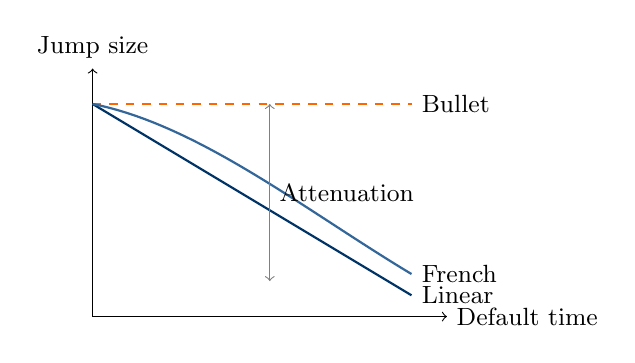
\begin{tikzpicture}[scale=0.9]
% Axes
\draw[->] (0,0) -- (5,0) node[right] {\small Default time};
\draw[->] (0,0) -- (0,3.5) node[above] {\small Jump size};

% Bullet (constant)
\draw[thick, orange, dashed] (0,3) -- (4.5,3) node[right, black] {\small Bullet};

% Linear (declining)
\draw[thick, darkblue] (0,3) -- (4.5,0.3) node[right, black] {\small Linear};

% French (convex decline)
\draw[thick, lightblue] (0,3) .. controls (1.5,2.7) and (3,1.5) .. (4.5,0.6) node[right, black] {\small French};

% Annotation
\draw[<->, gray] (2.5,0.5) -- (2.5,3) node[midway, right, black] {\small Attenuation};
\end{tikzpicture}
\end{center}

\vspace{0.5em}
\centering
\alert{Compounding effect:} Early defaults reduce intensity $\rightarrow$ fewer subsequent defaults
\end{column}
\end{columns}

\end{frame}

% ============================================================
% SECTION 3: EXPERIMENTAL DESIGN
% ============================================================
\section{Experimental Design}

\begin{frame}{Simulation Setup}

\begin{columns}[T]
\begin{column}{0.48\textwidth}
\textbf{Portfolio Parameters:}
\begin{itemize}
\item $N = 1{,}000$ obligors
\item $J = 3$ sectors
\item $X^A \sim \mathcal{U}[0.01, 0.03]$
\item Principal $P = 10$ each
\item Rate $r = 12\%$ annual
\end{itemize}

\vspace{1em}
\textbf{Sector Configurations:}
\begin{itemize}
\item \textbf{Balanced:} $w^{Aj} = 1/3$ all $j$
\item \textbf{Concentrated:} $w^{A,1} = 0.7$
\item \textbf{Mixed:} $(0.5, 0.3, 0.2)$
\end{itemize}

\vspace{1em}
\textbf{Contagion:} $c = 0.01$
\end{column}

\begin{column}{0.48\textwidth}
\textbf{Analysis Dimensions:}

\vspace{0.5em}
\begin{enumerate}
\item \textbf{Tail Risk} ($T=1$)
\begin{itemize}
\item Expected Shortfall
\item Value-at-Risk
\item Loss distributions
\end{itemize}

\vspace{0.5em}
\item \textbf{Survival Analysis} ($T=2$)
\begin{itemize}
\item First passage times
\item Threshold crossing probabilities
\end{itemize}

\vspace{0.5em}
\item \textbf{Contagion Mechanism}
\begin{itemize}
\item Peak intensity
\item Default clustering
\item Amplification factors
\end{itemize}
\end{enumerate}

\vspace{1em}
\textbf{Monte Carlo:} 2,500 paths\\
\textbf{Algorithm:} Giesecke-Kim-Zhu (2011)
\end{column}
\end{columns}

\end{frame}

% ============================================================
% SECTION 4: TAIL RISK RESULTS
% ============================================================
\section{Tail Risk Results}

\begin{frame}{Risk Metrics: Balanced Allocation}

\begin{table}
\centering
\small
\begin{tabular}{lccccc}
\toprule
\textbf{Schedule} & \textbf{Mean} & \textbf{Std Dev} & \textbf{VaR}$_{95}$ & \textbf{ES}$_{95}$ & \textbf{Excess ES} \\
\midrule
Bullet & 445.16 & 92.11 & 603.68 & \alert{653.19} & 49.51 \\
French & 192.02 & 39.74 & 260.42 & 282.88 & 22.46 \\
Linear & 187.92 & 39.41 & 254.87 & \alert{277.08} & 22.21 \\
\bottomrule
\end{tabular}
\end{table}

\vspace{1em}
\textbf{Key Finding:} Bullet ES is \alert{2.36$\times$} Linear ES

\vspace{1em}
\begin{columns}[T]
\begin{column}{0.48\textwidth}
\textbf{Observations:}
\begin{itemize}
\item Clear ordering across all metrics
\item French slightly higher than Linear
\item Excess ES: tail thickness beyond VaR
\end{itemize}
\end{column}

\begin{column}{0.48\textwidth}
\textbf{Mechanism:}
\begin{itemize}
\item Temporal alignment: intensity and EAD evaluated at same time
\item Late defaults $\rightarrow$ peak stress
\item Bullet: full exposure at peak
\item Amortizing: reduced exposure
\end{itemize}
\end{column}
\end{columns}

\end{frame}

\begin{frame}{Loss Distributions: Concentration Amplifies Tails}

\begin{columns}[c]
\begin{column}{0.48\textwidth}
\includegraphics[width=\textwidth]{figures/loss_conc.png}
\centering
\small Concentrated ($w^{A,1} = 0.7$)
\end{column}

\begin{column}{0.48\textwidth}
\includegraphics[width=\textwidth]{figures/loss_mixed.png}
\centering
\small Mixed $(0.5, 0.3, 0.2)$
\end{column}
\end{columns}

\vspace{1em}
\textbf{Asymmetric amplification:} Concentration extends Bullet tail disproportionately; amortizing schedules remain tight

\end{frame}

\begin{frame}{Expected Shortfall Across Configurations}

\begin{center}
\includegraphics[width=0.25\textwidth]{figures/es-summary.png}
\end{center}

\vspace{-0.5em}
\textbf{Three Critical Findings:}
\begin{enumerate}
\item \alert{Repayment structure dominates ES level:} Bullet/Linear ratio $\approx 2.3$ stable across all configurations
\item \alert{Concentration governs sensitivity:} Absolute gaps widen under Concentrated
\item \alert{Tail thickness structural:} Excess ES difference persists even with maximal diversification
\end{enumerate}

\end{frame}

% ============================================================
% SECTION 5: SURVIVAL ANALYSIS
% ============================================================
\section{Survival Analysis}

\begin{frame}{First Passage Time Framework}

\textbf{Question:} How quickly does portfolio reach systemic stress?

\vspace{1em}
\begin{columns}[T]
\begin{column}{0.48\textwidth}
\textbf{Aggregate intensity:}
\begin{equation*}
\mathcal{Y}_t = \sum_{j=1}^J Y^j_t
\end{equation*}

\textbf{First passage time:}
\begin{equation*}
\tau^\star = \inf\{t > 0 : \mathcal{Y}_t \geq y^\star\}
\end{equation*}

\textbf{Survival probability:}
\begin{equation*}
S(t) = \mathbb{P}(\tau^\star > t)
\end{equation*}
\end{column}

\begin{column}{0.48\textwidth}
\textbf{Why it matters:}
\begin{itemize}
\item Speed $\rightarrow$ intervention time
\item Early stress $\rightarrow$ no hedging
\item Deferred stress $\rightarrow$ risk management possible
\end{itemize}

\vspace{1em}
\textbf{Threshold:}
\begin{equation*}
y^\star_D = 0.75 \times \sum_j \lambda^j_{\max}
\end{equation*}

\vspace{0.5em}
\textbf{Horizon:} $T = 2$ (extended)
\end{column}
\end{columns}

\end{frame}

\begin{frame}{Mechanism: Amortization as Negative Feedback Brake}

\begin{center}
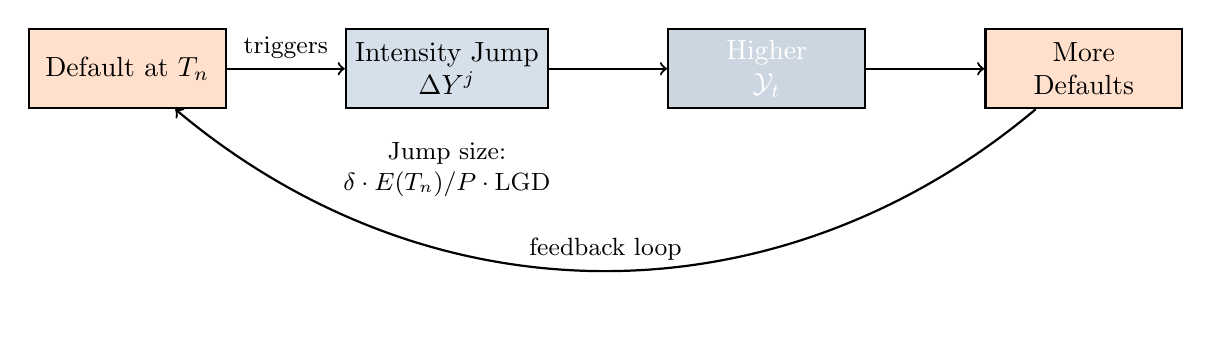
\begin{tikzpicture}[
    node distance=1.5cm,
    box/.style={rectangle, draw, thick, minimum width=2.5cm, minimum height=1cm, align=center},
    arrow/.style={->, thick}
]

% Nodes
\node[box, fill=orange!20] (default) {Default at $T_n$};
\node[box, fill=lightblue!20, right=of default] (jump) {Intensity Jump\\$\Delta Y^j$};
\node[box, fill=darkblue!20, text=white, right=of jump] (intensity) {Higher\\$\mathcal{Y}_t$};
\node[box, fill=orange!20, right=of intensity] (nextdef) {More\\Defaults};

% Arrows
\draw[arrow] (default) -- (jump) node[midway, above, font=\small] {triggers};
\draw[arrow] (jump) -- (intensity);
\draw[arrow] (intensity) -- (nextdef);
\draw[arrow, bend left=40] (nextdef) to node[midway, above, font=\small] {feedback loop} (default);

% Attenuation annotation
\node[below=0.3cm of jump, align=center, font=\small] {Jump size:\\$\delta \cdot \alert{E(T_n)/P} \cdot \text{LGD}$};

\end{tikzpicture}
\end{center}

\vspace{0.5em}
\begin{columns}[T]
\begin{column}{0.48\textwidth}
\textbf{Bullet:}
\begin{itemize}
\item $E(T_n)/P = 1$ always
\item No brake
\item Accelerating feedback
\end{itemize}
\end{column}

\begin{column}{0.48\textwidth}
\textbf{Amortizing:}
\begin{itemize}
\item $E(T_n)/P < 1$, declining
\item \alert{Brake applied}
\item Dampened feedback
\end{itemize}
\end{column}
\end{columns}

\vspace{1em}
\centering
Late defaults most attenuated $\rightarrow$ delays/prevents threshold crossing

\end{frame}

\begin{frame}{Survival Curves: Concentrated Allocation}

\begin{center}
\includegraphics[width=0.7\textwidth]{figures/survival_con_det.png}
\end{center}


\end{frame}
\begin{frame}{Survival Curves: Concentrated Allocation}
\vspace{-0.5em}
\begin{columns}[T]
\begin{column}{0.48\textwidth}
\textbf{Observations:}
\begin{itemize}
\item Bullet: rapid decline to near-zero
\item Amortizing: much slower decline
\item Gap widens over time
\end{itemize}
\end{column}

\begin{column}{0.48\textwidth}
\textbf{Concentration effects:}
\begin{itemize}
\item Accelerates all schedules
\item Bullet $\rightarrow$ almost certain crossing
\item Amortizing: protective effect \emph{strengthened}
\end{itemize}
\end{column}
\end{columns}

\end{frame}

\begin{frame}{First Passage Statistics}

\begin{table}
\centering
\begin{tabular}{llcc}
\toprule
\textbf{Sector} & \textbf{Schedule} & \textbf{Prob. Crossing} & \textbf{Mean Time} \\
& & $\hat{p}$ & $\hat{\mu}$ \\
\midrule
\multirow{3}{*}{Balanced} & Bullet & \alert{0.985} & 1.072 \\
& French & 0.174 & 1.057 \\
& Linear & \alert{0.129} & 1.071 \\
\midrule
\multirow{3}{*}{Concentrated} & Bullet & \alert{1.000} & 0.686 \\
& French & 0.854 & 0.878 \\
& Linear & \alert{0.799} & 0.879 \\
\bottomrule
\end{tabular}
\end{table}

\vspace{1em}
\textbf{Key Findings:}
\begin{itemize}
\item Under Balanced: 87\% of Linear paths \emph{never cross threshold}
\item Under Concentrated: All Bullet paths cross; 20\% of Linear paths survive
\item Conditional mean time: approximately equal for Linear/French, shorter for Bullet
\end{itemize}

\end{frame}

% ============================================================
% SECTION 6: CONTAGION MECHANISM
% ============================================================
\section{Contagion Mechanism}

\begin{frame}{Peak Intensity vs Total Loss}

\begin{center}
\includegraphics[width=0.7\textwidth]{figures/ymax_scatter.png}
\end{center}

\vspace{-0.5em}
\textbf{Key Insight:} Bullet clouds shifted both \alert{rightward} (higher loss) and \alert{upward} (higher peak intensity) with proportional alignment

\vspace{0.5em}
Amortizing: compressed clouds, shallower slope $\rightarrow$ reduced EAD limits loss even when intensity spikes

\end{frame}

\begin{frame}{Default Clustering: The Amplification Factor}

\textbf{Definition:}
\begin{equation*}
\mathcal{A} = \frac{\mathbb{E}[N(T) \mid L_T \geq \text{VaR}_{95}]}{\mathbb{E}[N(T)]}
\end{equation*}

Measures how much \emph{more} defaults occur in tail scenarios

\vspace{1em}
\begin{table}
\centering
\begin{tabular}{lcccc}
\toprule
\textbf{Schedule} & $\mathcal{Y}_{\max}^{(99)}$ & $\mathbb{E}[N]$ & $\mathbb{E}[N \mid \text{Tail}]$ & $\mathcal{A}$ \\
\midrule
Bullet & \alert{1.090} & 265.47 & 358.69 & \alert{1.351} \\
French & 0.560 & 191.15 & 259.19 & \alert{1.356} \\
Linear & \alert{0.529} & 186.63 & 247.82 & \alert{1.328} \\
\bottomrule
\end{tabular}
\end{table}

\vspace{1em}
\textbf{Striking Finding:} $\mathcal{A}$ essentially \alert{invariant} across schedules (1.33–1.36)

\end{frame}

\begin{frame}{Interpretation: Scale vs Clustering}

\begin{columns}[T]
\begin{column}{0.58\textwidth}
\textbf{What $\mathcal{A}$ tells us:}
\begin{itemize}
\item Measures \emph{relative} clustering
\item Governed by contagion parameter $c$
\item \alert{Not} affected by EAD profile
\end{itemize}

\vspace{1em}
\textbf{Implication:}
\begin{itemize}
\item Amortization is \alert{exposure scale parameter}
\item Does \emph{not} alter clustering structure
\item Attenuates \emph{every} loss proportionately
\end{itemize}

\vspace{1em}
\alert{Gap in $\mathbb{E}[N \mid \text{Tail}]$} (247 vs 359) entirely due to:
\begin{itemize}
\item Higher $\mathbb{E}[N]$ under Bullet
\item Elevated EAD amplifies each jump
\item Accelerates subsequent defaults
\end{itemize}
\end{column}

\begin{column}{0.38\textwidth}
\begin{center}
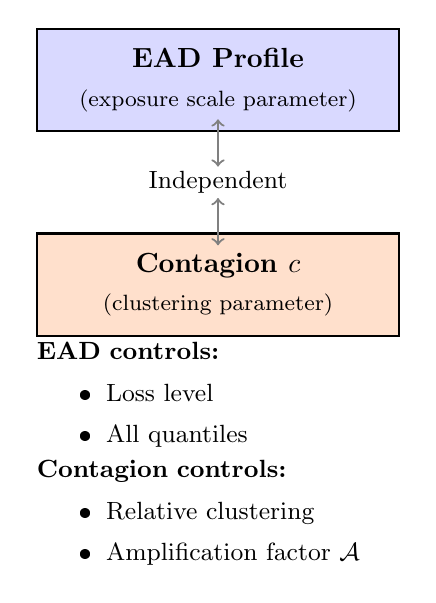
\begin{tikzpicture}[scale=1, every node/.style={transform shape}]

% ----------------------
% Main mechanism boxes
% ----------------------
\node[
  draw, thick, rectangle,
  minimum width=4.6cm,
  minimum height=1.3cm,
  fill=blue!15,
  align=center
] (ead) at (0,4.4)
{\textbf{EAD Profile}\\[2pt]
\footnotesize (exposure scale parameter)};

\node[
  draw, thick, rectangle,
  minimum width=4.6cm,
  minimum height=1.3cm,
  fill=orange!20,
  align=center
] (contagion) at (0,1.8)
{\textbf{Contagion $c$}\\[2pt]
\footnotesize (clustering parameter)};

% ----------------------
% Independence marker
% ----------------------
\node[
  font=\small
] at (0,3.1)
{Independent};

\draw[<->, thick, gray] (0,3.9) -- (0,3.3);
\draw[<->, thick, gray] (0,2.9) -- (0,2.3);

% ----------------------
% Explanatory blocks (stacked, narrow)
% ----------------------
\node[
  align=left,
  font=\small,
  text width=4.6cm
] at (0,0.4)
{\textbf{EAD controls:}
\begin{itemize}
  \item Loss level
  \item All quantiles
\end{itemize}
};

\node[
  align=left,
  font=\small,
  text width=4.6cm
] at (0,-1.1)
{\textbf{Contagion controls:}
\begin{itemize}
  \item Relative clustering
  \item Amplification factor $\mathcal{A}$
\end{itemize}
};

\end{tikzpicture}
\end{center}
\end{column}
\end{columns}

\end{frame}

% ============================================================
% SECTION 7: THEORETICAL FOUNDATION
% ============================================================
\section{Theoretical Foundation}

\begin{frame}{Risk Ordering: Coupling Argument}

\textbf{Setup:} Two portfolios with identical randomness but different EAD schedules:
\begin{equation*}
E^A_{\mathcal{P}_A}(t) \;\leq\; E^A_{\mathcal{P}_B}(t) \quad \forall\, A,\, t
\end{equation*}

\vspace{1em}
\begin{columns}[T]
\begin{column}{0.48\textwidth}
\textbf{Pathwise Dynamics:}
\begin{enumerate}
\item First default $T_1$ identical
\item Contagion jump: $\Delta \mathcal{Y}_{T_1}^B \geq \Delta \mathcal{Y}_{T_1}^A$
\item Intensity ordering propagates
\item More defaults in $\mathcal{P}_B$
\item Each with larger loss
\end{enumerate}
\end{column}

\begin{column}{0.48\textwidth}
\textbf{Result:}
\begin{align*}
L_T^{\mathcal{P}_B} &\geq_{\text{st}} L_T^{\mathcal{P}_A} \\
&\Downarrow \\
L_T^{\mathcal{P}_A} &\leq_{\text{cx}} L_T^{\mathcal{P}_B} \\
&\Downarrow \\
\text{ES}_\alpha(L_T^A) &\leq \text{ES}_\alpha(L_T^B)
\end{align*}

\vspace{0.5em}
Holds for all $\alpha \in (0,1)$
\end{column}
\end{columns}

\vspace{1em}
\textbf{Application:} $E_{\text{Linear}} \leq E_{\text{French}} \leq E_{\text{Bullet}} \leq E_{\text{Neg.Am.}}$

$\Rightarrow$ Heavy tails are \alert{intrinsic mathematical property}, not simulation artifact

\end{frame}

% ============================================================
% SECTION 8: POLICY IMPLICATIONS
% ============================================================
\section{Policy Implications}

\begin{frame}{Misspecification in Static Models}

\begin{columns}[T]
\begin{column}{0.48\textwidth}
\textbf{Standard Practice:}
\begin{itemize}
\item Treat all loans as zero-coupon bonds
\item Constant notional (Bullet schedule)
\item Compute capital requirements
\end{itemize}

\vspace{1em}
\textbf{Our Finding:}
\begin{equation*}
\text{ES}_{\text{Bullet}} \approx 2.3 \times \text{ES}_{\text{Linear}}
\end{equation*}

\vspace{0.5em}
Ratio \alert{stable across all concentration regimes}
\end{column}

\begin{column}{0.48\textwidth}
\textbf{Consequences:}

\vspace{0.5em}
\begin{itemize}
\item \textbf{Amortizing portfolio:}\\
Capital \alert{2$\times$ too high}

\vspace{0.5em}
\item \textbf{Negative Am. portfolio:}\\
Capital \alert{2$\times$ too low}

\vspace{0.5em}
\item Error \emph{not reduced} by diversification
\end{itemize}

\vspace{1em}
\alert{Recommendation:}\\
Explicitly model time-varying EAD in capital frameworks
\end{column}
\end{columns}

\end{frame}

\begin{frame}{Separation of Policy Levers}

\begin{center}
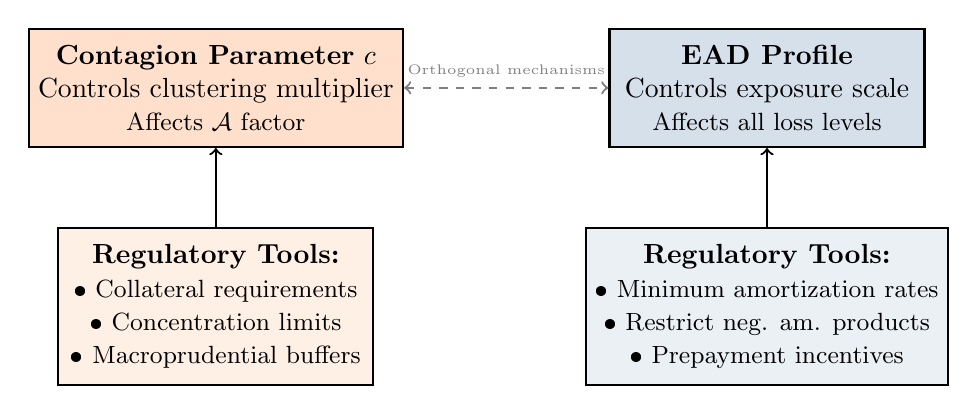
\begin{tikzpicture}[
    box/.style={rectangle, draw, thick, minimum width=4cm, minimum height=1.5cm, align=center},
    arrow/.style={->, thick}
]

% Two mechanisms
\node[box, fill=orange!20] (c) at (0,0) {\textbf{Contagion Parameter} $c$\\
Controls clustering multiplier\\
{\small Affects $\mathcal{A}$ factor}};

\node[box, fill=lightblue!20] (ead) at (7,0) {\textbf{EAD Profile}\\
Controls exposure scale\\
{\small Affects all loss levels}};

% Policy tools
\node[box, fill=orange!10, below=1cm of c, minimum height=2cm] (cpolicy) {
\textbf{Regulatory Tools:}\\
{\small • Collateral requirements}\\
{\small • Concentration limits}\\
{\small • Macroprudential buffers}
};

\node[box, fill=lightblue!10, below=1cm of ead, minimum height=2cm] (eadpolicy) {
\textbf{Regulatory Tools:}\\
{\small • Minimum amortization rates}\\
{\small • Restrict neg. am. products}\\
{\small • Prepayment incentives}
};

% Arrows
\draw[arrow] (cpolicy) -- (c);
\draw[arrow] (eadpolicy) -- (ead);

% Independence
\draw[<->, thick, gray, dashed] (c) -- (ead) node[midway, above] {\tiny Orthogonal mechanisms};

\end{tikzpicture}
\end{center}

\vspace{1em}
\textbf{Key Insight:} Diversification and amortization are \alert{complementary}, not substitutable

\end{frame}

% ============================================================
% SECTION 9: CONCLUSIONS
% ============================================================
\section{Conclusions}

\begin{frame}{Summary of Findings}

\textbf{Main Results:}

\vspace{0.5em}
\begin{enumerate}
\item \textbf{Repayment structure dominates tail risk}
\begin{itemize}
\item Bullet ES $\approx$ 2.3$\times$ Linear ES (stable across configurations)
\item Excess ES: Bullet tail events disproportionately severe
\end{itemize}

\vspace{0.5em}
\item \textbf{Amortization extends survival time}
\begin{itemize}
\item 87\% of Linear paths never reach stress threshold (Balanced)
\item Conditional mean FPT: Linear $\approx$ French $>$ Bullet
\item Protective effect \emph{strengthened} by concentration
\end{itemize}

\vspace{0.5em}
\item \textbf{Amplification Factor invariant to schedule}
\begin{itemize}
\item $\mathcal{A} \in [1.33, 1.36]$ across all schedules
\item Clustering governed by $c$, not EAD
\item Amortization = exposure scale parameter
\end{itemize}
\end{enumerate}

\end{frame}

\begin{frame}{Broader Implications}

\begin{columns}[T]
\begin{column}{0.48\textwidth}
\textbf{For Risk Management:}
\begin{itemize}
\item Static EAD models severely misspecify capital
\item Error magnitude: 2$\times$ (not marginal)
\item Applies to stress tests, ICAAP, CCAR
\end{itemize}

\vspace{1em}
\textbf{For Regulation:}
\begin{itemize}
\item Mandate EAD schedules in capital models
\item Separate levers for $c$ and EAD
\item Product restrictions (neg. am.) justified
\end{itemize}
\end{column}

\begin{column}{0.48\textwidth}
\textbf{For Portfolio Construction:}
\begin{itemize}
\item Amortization $\neq$ diversification
\item Both needed for tail risk reduction
\item Temporal dimension critical
\end{itemize}

\vspace{1em}
\textbf{Theoretical:}
\begin{itemize}
\item Convex ordering establishes rigorous foundation
\item Heavy tails intrinsic to deferred repayment
\item Negative feedback brake mechanism
\end{itemize}
\end{column}
\end{columns}

\vspace{1em}
\centering
\alert{Time-varying exposure is a first-order determinant of systemic credit risk}

\end{frame}

\begin{frame}{Future Directions}

\textbf{Extensions:}

\vspace{0.5em}
\begin{itemize}
\item \textbf{Heterogeneous maturities:} Maturity concentration as additional risk dimension

\vspace{0.5em}
\item \textbf{Prepayment optionality:} Effective EAD deviates from contractual when rates fall

\vspace{0.5em}
\item \textbf{Inter-sector contagion:} Cross-sector feedback beyond current framework

\vspace{0.5em}
\item \textbf{Stochastic recovery correlation:} LGD negatively correlated with default rates

\vspace{0.5em}
\item \textbf{Dynamic hedging strategies:} Optimal intervention given survival probabilities
\end{itemize}

\vspace{1em}
\textbf{Practical Applications:}
\begin{itemize}
\item Calibration to real bank portfolios
\item Stress testing frameworks
\item Product design and pricing
\end{itemize}

\end{frame}

% ============================================================
% THANK YOU
% ============================================================
\begin{frame}[plain]
\begin{center}
\vspace{2cm}
{\Huge Thank You}

\vspace{2cm}
{\Large Questions?}

\vspace{2cm}
\end{center}
\end{frame}

% ============================================================
% BACKUP SLIDES
% ============================================================
\appendix

\begin{frame}{Backup: Parameter Values}

\begin{table}
\centering
\small
\begin{tabular}{lll}
\toprule
\textbf{Parameter} & \textbf{Value} & \textbf{Description} \\
\midrule
\multicolumn{3}{l}{\textit{Portfolio}} \\
$N$ & 1,000 & Number of obligors \\
$J$ & 3 & Number of sectors \\
$P$ & 10 & Principal per loan \\
$T$ & 1 or 2 & Time horizon (years) \\
\midrule
\multicolumn{3}{l}{\textit{Intensity Dynamics}} \\
$X^A$ & $\mathcal{U}[0.01, 0.03]$ & Idiosyncratic intensity \\
$\kappa^j$ & 0.5 & Mean reversion speed \\
$\theta^j$ & 0.05 & Long-run mean \\
$\sigma^j$ & 0.15 & Volatility \\
$Y^j_0$ & 0.03 & Initial intensity \\
\midrule
\multicolumn{3}{l}{\textit{Contagion \& Recovery}} \\
$c$ & 0.01 & Base contagion strength \\
$\alpha$ & 4.5 & LGD Beta parameter \\
$\beta$ & 5.5 & LGD Beta parameter \\
\midrule
\multicolumn{3}{l}{\textit{Simulation}} \\
$M$ & 2,500 & Monte Carlo paths \\
\bottomrule
\end{tabular}
\end{table}

\end{frame}

\begin{frame}{Backup: Sector Weight Configurations}

\begin{table}
\centering
\begin{tabular}{lccc}
\toprule
\textbf{Configuration} & $w^{A,1}$ & $w^{A,2}$ & $w^{A,3}$ \\
\midrule
Balanced & 0.333 & 0.333 & 0.333 \\
Concentrated & 0.700 & 0.150 & 0.150 \\
Mixed & 0.500 & 0.300 & 0.200 \\
Random & \multicolumn{3}{c}{$\sim \text{Dirichlet}(1,1,1)$} \\
\bottomrule
\end{tabular}
\end{table}

\vspace{1em}
\textbf{Interpretation:}
\begin{itemize}
\item Balanced: Maximum diversification
\item Concentrated: Dominant sector absorbs 70\% exposure
\item Mixed: Partial concentration
\item Random: Each obligor draws weights from uniform Dirichlet
\end{itemize}

\end{frame}

% \begin{frame}{Backup: Monte Carlo Algorithm}

% \textbf{Giesecke-Kim-Zhu Acceptance-Rejection (2011):}

% \vspace{1em}
% \begin{enumerate}
% \item Set upper bounds $\lambda^j_{\max}$ on sectoral intensities

% \vspace{0.5em}
% \item Simulate candidate default times from Poisson process:
% \begin{equation*}
% \text{rate} = \sum_{j=1}^J \lambda^j_{\max}
% \end{equation*}

% \vspace{0.5em}
% \item At each candidate time:
% \begin{itemize}
% \item Accept/reject based on $\lambda_t / \lambda_{\max}$
% \item If accepted: sample defaulting obligor proportionally to $\lambda^A_t$
% \end{itemize}

% \vspace{0.5em}
% \item Upon acceptance:
% \begin{itemize}
% \item Draw $\text{LGD}^A \sim \text{Beta}(4.5, 5.5)$
% \item Compute loss: $\ell^A = \text{LGD}^A \cdot E^A(t)$
% \item Update intensities: $\Delta Y^j = \delta^{Aj} \ell^A / P^A$
% \end{itemize}

% \vspace{0.5em}
% \item Continue until horizon $T$
% \end{enumerate}

% \vspace{0.5em}
% \textbf{Properties:} Asymptotically exact, computationally efficient

% \end{frame}

% ============================================================
% BIBLIOGRAPHY
% ============================================================
\begin{frame}[allowframebreaks]{References}

\begin{thebibliography}{99}

\bibitem{sinha2025}
D.~Sinha, S.~Sharma, S.~Jain, and S.~K.~Iyer,
``Simulation and Analysis of Sector-Apportioned Intensity Models for Correlated Defaults,''
\textit{Working Paper}, 2025.

\bibitem{giesecke2011}
K.~Giesecke, B.~Kim, and S.~Zhu,
``Monte Carlo Algorithms for Default Timing Problems,''
\textit{Management Science}, vol.~57, no.~12, pp.~2115--2129, 2011.

\end{thebibliography}

\end{frame}

\end{document}